\documentclass{beamer}
\usepackage{amsmath}
\usepackage{amsfonts}
\usepackage{mathrsfs}
\usepackage{amssymb}
\usepackage{graphicx} % 插入图形
\usepackage{enumerate}
\usepackage{datetime}
\usepackage{paralist}
\usepackage{color}
\usepackage{float}
\usepackage{nicematrix}
\usepackage{tikz}
\usetikzlibrary{matrix,decorations.pathreplacing}
\usepackage{arydshln}%虚线
\usepackage{algorithm} % 算法
\usepackage{algmatlab}


\usepackage[utf8]{inputenc}
% \usepackage{amsmath,amssymb}
% \usepackage{graphicx}
\usepackage{biblatex}
\usepackage{hyperref}

% 主题设置
\usetheme{Madrid}
\usecolortheme{seahorse}
\usefonttheme{serif}

% 标题页信息
\title{QR Decomposition for Split Quaternion Matrices}
\subtitle{Theoretical Development and Algorithmic Implementation}
\author{Liu Qianqian \\ \small Macau University of Science and Technology}
% \institute{Faculty of Innovation Engineering, Macau University of Science and Technology, Avenida Wai Long, TaiPa, Macau}
\date{\today}

% 参考文献设置
\addbibresource{references.bib} % 假设你的bib文件名为references.bib

\begin{document}

% 标题页
\begin{frame}
  \titlepage
\end{frame}

% 目录页
% \begin{frame}{Outline}
%   \tableofcontents
% \end{frame}
\begin{frame}{abstract}
Split quaternion algebra is not a Euclidean distance space because of having zero divisors. Thus, the traditional QR decomposition based on Givens rotations and Householder reflection transformations is difficult to implement. To overcome this difficulty and to address the non-commutativity of split quaternion multiplication, we utilize the real representation $A^\sigma$ of the split quaternion matrix $A$. By leveraging the proposed decomposition $A^\sigma = \widetilde{Q}R_4$ ($\widetilde{Q}$ is an orthogonal matrix, and $R_4 = \begin{bmatrix} R_{11} & R_{12} \\ R_{21} & R_{22} \end{bmatrix}$ with $R_{11}, R_{12}, R_{21}, R_{22}$ being upper triangular), the QR decomposition of $A$ is successfully constructed and the corresponding algorithms are developed.The experimental results show that it performs well in both speed and accuracy.
\end{frame}
% 引言部分
% \section{Introduction}
\begin{frame}{Introduction}
  In 1849, James Cockle \cite{Cockle1849} introduced the concept of split quaternion algebra over the real number field $\mathbb{R}$, defined as:
  \begin{equation*}
    \mathbb{H}_s = \left\{ a_0 + a_1 i + a_2 j + a_3 k \ \bigg| \ 
     \ a_0, a_1, a_2, a_3 \in \mathbb{R}
    \right\}.
  \end{equation*}
where
   \begin{equation*}
       i^2 = -1,\ j^2 = k^2 = 1,  \ ijk = 1,
   \end{equation*}
\end{frame}

\begin{frame}{Properties of Split Quaternions}
  $\mathbb{H}_s$ is a:
  \begin{itemize}
    \item Four-dimensional algebra
    \item Non-commutative algebra
    \item Algebra containing zero divisors
  \end{itemize}
  
  \vspace{1em}
  Many studies on split quaternions:
  \begin{itemize}
    \item Algebraic properties \cite{AR2020,Yasemin2012,TJiang2015,Jiang2018}
    \item Applications in quantum mechanics, electromagnetism, signal processing \cite{Gog2022, Hasebe2010}
  \end{itemize}
\end{frame}
\begin{frame}{Previous Work}
We acknowledge that the split quaternion algebra does not constitute an Euclidean space, rendering traditional Givens rotations and Householder reflections inapplicable when applied to split quaternion vectors. This poses a substantial challenge for the conventional QR decomposition process for split quaternion matrices.

To address the above problem, we intend to utilize the real representation of split quaternions.
\end{frame}

\begin{frame}{Previous Work}
  Significant contributions include:
  \begin{itemize}
    \item Eigenvalue problem of split quaternion matrices \cite{Jiang2018}
    \item Solving classical systems of matrix equations \cite{wang2024}
    \item Fast algorithm for LDU decomposition \cite{Wang2021}
    \item Efficient algorithm for SVD \cite{Gang2024}
  \end{itemize}
  
  \vspace{1em}
  \alert{Research Gap:} QR decomposition for split quaternion matrices remains underdeveloped
\end{frame}

\begin{frame}{Challenges}
  \begin{block}{Key Challenge}
    The split quaternion algebra
    The split quaternion algebra does not constitute an Euclidean space, rendering traditional Givens rotations and Householder reflections inapplicable.
  \end{block}
  
  This poses a substantial challenge for conventional QR decomposition processes.
\end{frame}

\begin{frame}{Our Approach}
  To address this problem, we utilize the real representation of split quaternions:
  
  \begin{itemize}
    \item Multiple forms of real representations exist \cite{Zhuo2020, Yang2020, Xin2019, Gang2024}
    \item We use the $2m \times 2n$ compact real representation from \cite{Gang2024}
    \item Converts split quaternion decomposition to real matrix decomposition
  \end{itemize}
\end{frame}

\begin{frame}{Our Contributions}
  \begin{enumerate}
    \item Constructive proof of the existence of QR decomposition for split quaternion matrices
    \item Novel and efficient algorithm for computing QR decomposition
    \item Experimental validation of efficiency and accuracy
  \end{enumerate}
\end{frame}

\begin{frame}{Paper Organization}
  \begin{enumerate}
    \item \textbf{Section 2:} Real representation of split quaternion matrices and properties
    \item \textbf{Section 3:} Existence proof of QR decomposition, algorithm, and complexity analysis
    \item \textbf{Section 4:} Numerical examples and applications
    \item \textbf{Section 5:} Conclusions and future work
  \end{enumerate}
\end{frame}

% 标题页
% \begin{frame}
%     \title{Preliminaries on Split Quaternion Matrices}
% \end{frame}

% 基本定义1
\begin{frame}
    \frametitle{Basic Definitions}
    For a split quaternion matrix 
    \[
    A = A_0 + A_1i + A_2j + A_3k \in \mathbb{H}_s^{m \times n}
    \]
    where \(A_i \in \mathbb{R}^{m \times n}\) (\(i = 0,1,2,3\)), we define:
    \begin{itemize}
        \item Transpose: \(A^T = A_0^T + A_1^Ti + A_2^Tj + A_3^Tk\)
        \item Conjugate: \(\bar{A} = A_0 - A_1i - A_2j - A_3k\)
        \item Conjugate transpose: \(A^* = A_0^T - A_1^Ti - A_2^Tj - A_3^Tk\)
        \item i-conjugate: \(\tilde{A} = A_0 - A_1i + A_2j + A_3k\)
        \item i-conjugate transpose: \(A^H = A_0^T - A_1^Ti + A_2^Tj + A_3^Tk\)
    \end{itemize}
\end{frame}

% 实表示矩阵
\begin{frame}
    \frametitle{Real Representation Matrix}
    The real representation matrix of \(A \in \mathbb{H}_s^{m \times n}\) is:
    \begin{equation}
    A^\sigma = \begin{bmatrix} A_0 + A_2 & -A_1 + A_3 \\ A_1 + A_3 & A_0 - A_2 \end{bmatrix} \in \mathbb{R}^{2m \times 2n}
    \end{equation}
    \vspace{0.5cm}
    \textbf{Reference:} \cite{TJiang2018, Gang2024}
\end{frame}

% 性质
\begin{frame}
    \frametitle{Properties of Real Representation}
    For \(A, B \in \mathbb{H}_s^{m \times n}\), \(C \in \mathbb{H}_s^{n \times p}\), \(a \in \mathbb{R}\):
    \begin{equation}
    \begin{split}
    &(A + B)^\sigma = A^\sigma + B^\sigma, \quad (AC)^\sigma = A^\sigma C^\sigma, \\
    &(a A)^\sigma = a A^\sigma, \quad (A^H)^\sigma = (A^\sigma)^T
    \end{split}
    \end{equation}
\end{frame}

% 逆对应
\begin{frame}
    \frametitle{Inverse Correspondence}
    For a real matrix \(B = \begin{bmatrix} B_{11} & B_{12} \\ B_{21} & B_{22} \end{bmatrix} \in \mathbb{R}^{2m \times 2n}\) (\(B_{ts} \in \mathbb{R}^{m \times n}\)), the corresponding split quaternion matrix is:
    \begin{equation}
    A = \frac{B_{11} + B_{22}}{2} + \frac{B_{21} - B_{12}}{2}i + \frac{B_{11} - B_{22}}{2}j + \frac{B_{21} + B_{12}}{2}k
    \end{equation}
    where \(A^\sigma = B\), establishing a one-to-one mapping \cite{Gang2024}.
\end{frame}

% 酉矩阵与范数
\begin{frame}
    \frametitle{Unitary Matrices and Frobenius Norm}
    \begin{itemize}
        \item A matrix \(A\) is \textit{unitary} if \(AA^H = A^H A = I\)
        \item \(A\) is unitary \(\iff\) \(A^\sigma\) is orthogonal
        \item Frobenius norm of \(A\):
        \[
        \|A\|_F \equiv \frac{1}{\sqrt{2}} \|A^\sigma\|_F = \sqrt{\|A_0\|_F^2 + \|A_1\|_F^2 + \|A_2\|_F^2 + \|A_3\|_F^2}
        \]
    \end{itemize}
\end{frame}

% 范数不变性
% \begin{frame}
%     \frametitle{Norm Invariance Under Unitary Transformations}
%     If \(U\) and \(V\) are unitary, then \(U^\sigma\) and \(V^\sigma\) are orthogonal, and:
%     \[
%     \|UAV\|_F = \frac{1}{\sqrt{2}} \|(UAV)^\sigma\|_F 
%     = \frac{1}{\sqrt{2}} \|U^\sigma A^\sigma V^\sigma\|_F 
%     = \frac{1}{\sqrt{2}} \|A^\sigma\|_F 
%     = \|A\|_F
%     \]
%     Thus, the Frobenius norm is invariant under unitary transformations.
% \end{frame}

% % 标题页
% \begin{frame}
%     \title{QR Decomposition of Split Quaternion Matrices}
% \end{frame}

% 概述
\begin{frame}
    \frametitle{QR Decomposition of Split Quaternion Matrices}
    For \( A \in \mathbb{H}_s^{m \times n} \), QR decomposition is achieved via a two-step process:
    \begin{enumerate}
        \item \textbf{Step 1:} Construct a special decomposition of the real representation \( A^\sigma \):
        \[
        A^\sigma = \widetilde{Q} R_4
        \]
        where \( \widetilde{Q} \in \mathbb{R}^{2m \times 2m} \) is orthogonal, and \( R_4 \) is in the form of 
\begin{equation}\label{r4}
R_4 = \begin{bmatrix}
    R_{11} & R_{12} \\
    R_{21} & R_{22}
\end{bmatrix} \in \mathbb{R}^{2m \times 2n},
\end{equation}
and $R_{11}, R_{12},R_{21},R_{22}$ are all upper triangular matrices of size $m \times n$.
        \item \textbf{Step 2:} Construct split quaternion matrices \( Q \) (unitary) and \( R \) (upper triangular) such that \( A = QR \).
    \end{enumerate}
\end{frame}

% Step 1: 构造R4 - 行置换
\begin{frame}
    \frametitle{Step 1: Constructing \( R_4 \) (Row Permutations)}
    To transform an upper triangular \( R \in \mathbb{R}^{2m \times 2n} \) into \( R_4 \), first perform row permutations:
    \begin{enumerate}
\item Swap its rows $r_i$ as follows:  
   \begin{equation} \label{eq:rowswap}
       r_2 \leftrightarrow r_{m + 1 + (m \bmod 2)}, \quad r_4 \leftrightarrow r_{m + 3 + (m \bmod 2)}, \quad \dots.
   \end{equation}
\item  Partition into \( R_{\text{upper}} \in \mathbb{R}^{m \times 2n} \) and \( R_{\text{lower}} \in \mathbb{R}^{m \times 2n} \). If \( m \) is odd, append a zero row to the end of the last row of \( R_{\text{upper}} \) and prepend a zero row to the beginning of the first row of \( R_{\text{lower}} \) ensuring that the parity of each row index remains unchanged before the swap, the position of the zero row stays fixed after the swap, and further partitioning is possible.
 
\item Repeat steps 1 and 2 for \( R_{\text{upper}} \) and \( R_{\text{lower}} \) until all  partitioned submatrices contain exactly 2 rows.  
 
\item  Remove the added zero rows in step 2 to keep the same size.
\end{enumerate}
\end{frame}

% 行置换示例
\begin{frame}
    \frametitle{Row Permutation Example}
    To better understand the procedure, we choose the following matrix 
\[R= \begin{bmatrix}
 r_{11} & r_{12} & r_{13} & r_{14} & r_{15} & r_{16} & r_{17} & r_{18}\\
 0      & r_{22} & r_{23} & r_{24} & r_{25} & r_{26} & r_{27} & r_{28}\\
 0      & 0      & r_{33} & r_{34} & r_{35} & r_{36} & r_{37} & r_{38}\\
 0      & 0      & 0      & r_{44} & r_{45} & r_{46} & r_{47} & r_{48}\\
 0      & 0      & 0      & 0      & r_{55} & r_{56} & r_{57} & r_{58}\\
 0      & 0      & 0      & 0      & 0      & r_{66} & r_{67} & r_{68}\\
\end{bmatrix} \in \mathbb{R}^{2\cdot 3 \times 2 \cdot 4}
\]
    to show how the row/column transformations work. 
\end{frame}

\begin{frame}
    \frametitle{Row Permutation Example}
\begin{align*}
R =
  &\begin{bmatrix}
 r_{11} & r_{12} & r_{13} & r_{14} & r_{15} & r_{16} & r_{17} & r_{18}\\
 0      & r_{22} & r_{23} & r_{24} & r_{25} & r_{26} & r_{27} & r_{28}\\
 0      & 0      & r_{33} & r_{34} & r_{35} & r_{36} & r_{37} & r_{38}\\
 0      & 0      & 0      & r_{44} & r_{45} & r_{46} & r_{47} & r_{48}\\
 0      & 0      & 0      & 0      & r_{55} & r_{56} & r_{57} & r_{58}\\
 0      & 0      & 0      & 0      & 0      & r_{66} & r_{67} & r_{68}\\
\end{bmatrix}\\
\xrightarrow{r_{2} \leftrightarrow r_{5}}
&\begin{bmatrix}
% \begin{array}{cc:cc:cc}
 r_{11} & r_{12} & r_{13} & r_{14} & r_{15} & r_{16} & r_{17} & r_{18}\\
 0      & 0      & 0      & 0      & r_{55} & r_{56} & r_{57} & r_{58}\\
 0      & 0      & r_{33} & r_{34} & r_{35} & r_{36} & r_{37} & r_{38}\\
 % \cdashline{1-8}
 0      & 0      & 0      & r_{44} & r_{45} & r_{46} & r_{47} & r_{48}\\
 0      & r_{22} & r_{23} & r_{24} & r_{25} & r_{26} & r_{27} & r_{28}\\
 0      & 0      & 0      & 0      & 0      & r_{66} & r_{67} & r_{68}\\
% \end{array}
\end{bmatrix}
\end{align*}
\end{frame}

\begin{frame}{Row Permutation Example}
    % \frametitle{Row Permutation Example}
partition it into \ $R_{upper}, \ R_{lower}$:
    
     \begin{align*}
     % \xrightarrow{partition it into \ R_{upper}, \ R_{lower}}
 \small
 \begin{bmatrix}
 r_{11} & r_{12} & r_{13} & r_{14} & r_{15} & r_{16} & r_{17} & r_{18}\\
 0      & 0      & 0      & 0      & r_{55} & r_{56} & r_{57} & r_{58}\\
 0      & 0      & r_{33} & r_{34} & r_{35} & r_{36} & r_{37} & r_{38}\\
 \cdashline{1-8}
 0      & 0      & 0      & r_{44} & r_{45} & r_{46} & r_{47} & r_{48}\\
 0      & r_{22}  & r_{23} & r_{24} & r_{25} & r_{26} & r_{27} & r_{28}\\
 0      & 0      & 0      & 0      & 0      & r_{66} & r_{67} & r_{68}\\
\end{bmatrix}
\end{align*}
prepend zero rows of \( R_{upper} \) and \( R_{lower} \):
\begin{align*}
\small
\begin{bmatrix}
 r_{11} & r_{12} & r_{13} & r_{14} & r_{15} & r_{16} & r_{17} & r_{18}\\
 0      & 0      & 0      & 0      & r_{55} & r_{56} & r_{57} & r_{58}\\
 0      & 0      & r_{33} & r_{34} & r_{35} & r_{36} & r_{37} & r_{38}\\
 0      & 0      & 0      & 0      & 0      & 0      & 0      & 0     \\
 \cdashline{1-8}
 0      & 0      & 0      & 0      & 0      & 0      & 0      & 0     \\
 0      & 0      & 0      & r_{44} & r_{45} & r_{46} & r_{47} & r_{48}\\
 0      & r_{22} & r_{23} & r_{24} & r_{25} & r_{26} & r_{27} & r_{28}\\
 0      & 0      & 0      & 0      & 0      & r_{66} & r_{67} & r_{68}\\
\end{bmatrix} 
\end{align*}
\end{frame}

\begin{frame}{Frame Title}
    perform row swaps on $R_{upper}, \ R_{lower}$ and remove the added zero rows:
    \begin{align*}
\xrightarrow[r_{2} \leftrightarrow r_{3}\ on\ R_{lower}]{r_{2} \leftrightarrow r_{3}\ on\ R_{upper}}
&\begin{bmatrix}
 r_{11} & r_{12} & r_{13} & r_{14} & r_{15} & r_{16} & r_{17} & r_{18}\\
 0      & 0      & r_{33} & r_{34} & r_{35} & r_{36} & r_{37} & r_{38}\\
 0      & 0      & 0      & 0      & r_{55} & r_{56} & r_{57} & r_{58}\\
 0      & 0      & 0      & 0      & 0      & 0      &  0     & 0     \\
\cdashline{1-8}
 0      & 0      & 0      & 0      & 0      & 0      & 0      & 0     \\
 0      & r_{22} & r_{23} & r_{24} & r_{25} & r_{26} & r_{27} & r_{28}\\
 0      & 0      & 0      & r_{44} & r_{45} & r_{46} & r_{47} & r_{48}\\
 0      & 0      & 0      & 0      & 0      & r_{66} & r_{67} & r_{68}\\
\end{bmatrix}
\end{align*}\\
\begin{align*}
\xrightarrow {remove\ zero\ rows}
&\begin{bmatrix}
 r_{11} & r_{12} & r_{13} & r_{14} & r_{15} & r_{16} & r_{17} & r_{18}\\
 0      & 0      & r_{33} & r_{34} & r_{35} & r_{36} & r_{37} & r_{38}\\
 0      & 0      & 0      & 0      & r_{55} & r_{56} & r_{57} & r_{58}\\
 0      & r_{22} & r_{23} & r_{24} & r_{25} & r_{26} & r_{27} & r_{28}\\
 0      & 0      & 0      & r_{44} & r_{45} & r_{46} & r_{47} & r_{48}\\
 0      & 0      & 0      & 0      & 0      & r_{66} & r_{67} & r_{68}\\
\end{bmatrix}
\end{align*}
\end{frame}

% Step 1: 列置换
\begin{frame}
    \frametitle{Step 1: Constructing \( R_4 \) (Column Permutations)}
    After row permutations, perform column permutations:
    \begin{enumerate}
        \item Swap even columns with specific odd columns in the right half:
        \[
        c_2 \leftrightarrow c_{n + 1 + (n \bmod 2)},\ c_4 \leftrightarrow c_{n + 3 + (n \bmod 2)},\ \dots
        \]
        \item Partition into \( R_{\text{left}} \in \mathbb{R}^{2m \times n} \) and \( R_{\text{right}} \in \mathbb{R}^{2m \times n} \). If \( n \) is odd, add zero columns to maintain parity.
        \item Recursively apply to submatrices until all have 2 columns, then remove zero columns.
    \end{enumerate}
    Result: \( R_4 = \begin{bmatrix} R_{11} & R_{12} \\ R_{21} & R_{22} \end{bmatrix} \) with upper triangular blocks.
\end{frame}

\begin{frame}{Step 1: Constructing \( R_4 \) (Column Permutations)}
    \begin{enumerate}
\item For the columns \( c_i \) of the resulting matrix, we swap as follows:  
   \begin{equation} \label{eq:cswap}
       c_2 \leftrightarrow c_{n + 1 + (n \bmod 2)}, \quad c_4 \leftrightarrow c_{n + 3 + (n \bmod 2)}, \quad \dots.
   \end{equation}  
\item  Partition into  \( R_{\text{left}} \in \mathbb{R}^{2m \times n} \)  and  \( R_{\text{right}} \in \mathbb{R}^{2m \times n} \). If \( n \) is odd, append a zero column to the end of the last column of \( R_{\text{left}} \) and prepend a zero column to the beginning of the first column of \( R_{\text{right}} \), ensuring that the parity of each column index remains unchanged before the swap, the position of the zero column stays fixed after the swap, and further partitioning is possible.  
 
\item  Repeat steps 1 and 2 for \( R_{\text{left}} \) and \( R_{\text{right}} \) until all partitioned submatrices contain exactly 2 columns. 
 
\item Remove the added zero columns in step 2 to keep the same size.
\end{enumerate}
\end{frame}

% 列置换示例
\begin{frame}
    \frametitle{Column Permutation Example (Continued)}
    After row permutations, apply column swaps:
    \[
    \xrightarrow{c_2 \leftrightarrow c_5}
    \begin{bmatrix}
    r_{11} & r_{15} & r_{13} & r_{14} & r_{12} & \cdots \\
    0 & r_{35} & r_{33} & r_{34} & 0 & \cdots \\
    \vdots & \vdots & \vdots & \vdots & \vdots & \ddots
    \end{bmatrix}
    \xrightarrow{c_4 \leftrightarrow c_7}
    \begin{bmatrix}
    r_{11} & r_{15} & r_{13} & r_{17} & r_{12} & \cdots \\
    0 & r_{35} & r_{33} & r_{37} & 0 & \cdots \\
    \vdots & \vdots & \vdots & \vdots & \vdots & \ddots
    \end{bmatrix}
    \]
    Recursively swap columns in submatrices, resulting in:
    \[
    R_4 = \begin{bmatrix} R_{11} & R_{12} \\ R_{21} & R_{22} \end{bmatrix}
    \]
\end{frame}

% 置换矩阵P与算法1
\begin{frame}
    \frametitle{Permutation Matrix \( P_{2k} \)}
    The permutation matrix \( P_{2k} \) (orthogonal) enables the transformation \( P_{2m} R P_{2n}^T = R_4 \):
    \[
    P_{2k} = \begin{bmatrix} 
    1 & 0 & \cdots & 0 \\ 
    0 & 0 & 1 & \cdots \\ 
    \vdots & \vdots & \vdots & \ddots \\ 
    0 & 1 & 0 & \cdots \\ 
    \vdots & \vdots & \vdots & \ddots 
    \end{bmatrix}_{2k \times 2k}
    \]
\end{frame}
\iffalse
\begin{frame}
\frametitle{Matrix Permutation Recursive Algorithm}
    \small % 缩小字体避免过宽
    \begin{algorithm}[H] % 使用[H]固定位置避免浮动问题
    \caption{Matrix Permutation Recursive Algorithm} \label{alg:Permutation}
    \begin{algorithmic}[1]
    \Function{Permutation}{$P$}
        \State \% \textbf{Input:} \text{\textit{$P \in \mathbb{R}^{2s \times 2n}$, the matrix to permute.}}
        \State \% \textbf{Output:} \text{\textit{$P \in \mathbb{R}^{2s \times 2n}$, the matrix after permutation.}}
        \State
        \State \% \textbf{Step 1} \text{\textit{Recursive stop when $s=1$.}}
        \If{$s=1$}
            \State \Return $P$;
        \EndIf % 修正为\EndIf
        \State
        \State \% \textbf{Step 2} \text{\textit{Initialize $s2$.}}
        \State $s2 = \lfloor s/2 \rfloor$; % 使用正确的floor符号\lfloor\rfloor
        \State
        \State \% \textbf{Step 3} \text{\textit{Swap even rows in the upper half of $P$ with odd rows in the lower half of $P$.}}
        \For{$i=1:s2$}
            \If{$\mod(s, 2)=0$}
                \State $P = \operatorname{swap}(P, 2i, s+2i-1)$; % 使用\operatorname定义函数
            \Else
                \State $P = \operatorname{swap}(P, 2i, s+2i)$;
            \EndIf % 修正为\EndIf
        \EndFor % 修正为\EndFor
        \State
        \State \% \textbf{Step 4} \text{\textit{Partition matrix. Add zero rows, if $s$ is odd.}}
        \If{$\mod(s, 2)=1$}
            \State $P_{\text{upper}} = [P(1:s,:); \operatorname{zeros}(1, 2n)]$;
            \State $P_{\text{lower}} = [\operatorname{zeros}(1, 2n); P(s+1:\text{end})]$;
        \Else
            \State $P_{\text{upper}} = P(1:s,:)$;
            \State $P_{\text{lower}} = P(s+1:\text{end})$;
        \EndIf % 修正为\EndIf
        \State
        \State \% \textbf{Step 5} \text{\textit{Recursive execution.}}
        \State $P_{\text{upper}} = \Call{Permutation}{P_{\text{upper}}}$; % 使用\Call调用函数
        \State $P_{\text{lower}} = \Call{Permutation}{$P_{\text{lower}}$}$;
        \State
        \State \% \textbf{Step 6} \text{\textit{Remove zero rows, if $s$ is odd.}}
        \If{$\mod(s, 2)=1$}
            \State $P(1:s) = P_{\text{upper}}(1:s, :)$;
            \State $P(s+1:\text{end}) = P_{\text{lower}}(2:\text{end}, :)$;
        \Else
            \State $P(1:s) = P_{\text{upper}}(1:\text{end}, :)$;
            \State $P(s+1:\text{end}) = P_{\text{lower}}(1:\text{end}, :)$;
        \EndIf % 修正为\EndIf
    \EndFunction % 修正为\EndFunction
    \end{algorithmic}
    \end{algorithm}
\end{frame}

% 优化置换算法
\begin{frame}
    \frametitle{Optimized Permutation Algorithm}
    To reduce computational cost, use \text{PermutationOpt} to avoid matrix multiplications:
    \begin{algorithm}[H]
        \caption{Matrix Permutation Optimization Algorithm}
        \begin{algorithmic}[1]
        \Function{PermutationOpt}{$A,t$}
            \If{$t==0$} \Comment{Compute $B=P_{2m}AP_{2n}^T$}
                \For{$i=1:m$} $A_{\text{tmp}}(i,:)=A(2i-1,:)$; $A_{\text{tmp}}(m+i,:)=A(2i,:)$ \EndFor
                \For{$i=1:n$} $B(:,i)=A_{\text{tmp}}(:,2i-1)$; $B(:,n+i)=A_{\text{tmp}}(:,2i)$ \EndFor
            \Else \Comment{Compute $B=P_{2m}^TAP_{2n}$}
                \For{$i=1:m$} $A_{\text{tmp}}(2i-1,:)=A(i,:)$; $A_{\text{tmp}}(2i,:)=A(m+i,:)$ \EndFor
                \For{$i=1:n$} $B(:,2i-1)=A_{\text{tmp}}(:,i)$; $B(:,2i)=A_{\text{tmp}}(:,n+i)$ \EndFor
            \EndIf
            \Return $B$
        \EndFunction
        \end{algorithmic}
    \end{algorithm}
\end{frame}
\fi

% Step 2: 构造Q和R
\begin{frame}
    \frametitle{Step 2: Constructing \( Q \) and \( R \)}
    Using the real representation correspondence:
    \begin{itemize}
        \item For \( R_4 = \begin{bmatrix} R_{11} & R_{12} \\ R_{21} & R_{22} \end{bmatrix} \), construct upper triangular \( R \in \mathbb{H}_s^{m \times n} \):
        \[
        R = \frac{R_{11}+R_{22}}{2} + \frac{R_{21}-R_{12}}{2}i + \frac{R_{11}-R_{22}}{2}j + \frac{R_{21}+R_{12}}{2}k
        \]
        \item For orthogonal \( \widetilde{Q} = \begin{bmatrix} Q_{11} & Q_{12} \\ Q_{21} & Q_{22} \end{bmatrix} \), construct unitary \( Q \in \mathbb{H}_s^{m \times m} \):
        \[
        Q = \frac{Q_{11}+Q_{22}}{2} + \frac{Q_{21}-Q_{12}}{2}i + \frac{Q_{11}-Q_{22}}{2}j + \frac{Q_{21}+Q_{12}}{2}k
        \]
        \item Result: \( A = QR \) (since \( A^\sigma = Q^\sigma R^\sigma \)).
    \end{itemize}
\end{frame}

\iffalse
% QR分解算法
\begin{frame}
    \frametitle{QR Decomposition Algorithm for Split Quaternion Matrices}
    \begin{algorithm}[H]
        \caption{Compute QR of Split Quaternion Matrix \( A \)}
        \begin{algorithmic}[1]
        \Function{Split-QR}{$A$}
            \State \% Step 1: Real representation of $A$
            \State $A^\sigma = \begin{bmatrix} A_0+A_2 & -A_1+A_3 \\ A_1+A_3 & A_0-A_2 \end{bmatrix}$
            \State \% Step 2: Permute $A^\sigma$
            \State $\widehat{A} = \text{PermutationOpt}(A^\sigma, 1)$
            \State \% Step 3: QR decomposition of $\widehat{A}$
            \State $[\widehat{Q}, \widehat{R}] = \text{qr}(\widehat{A})$
            \State \% Step 4: Recover $R^\sigma$ and $Q^\sigma$
            \State $R^\sigma = \text{PermutationOpt}(\widehat{R}, 0)$
            \State $Q^\sigma = \text{PermutationOpt}(\widehat{Q}, 0)$
            \State \% Step 5: Construct $Q$ and $R$ (split quaternion)
            \State Compute $Q_0,Q_1,Q_2,Q_3$ and $R_0,R_1,R_2,R_3$ from blocks
            \State $Q = Q_0 + Q_1i + Q_2j + Q_3k$; $R = R_0 + R_1i + R_2j + R_3k$
            \Return $Q, R$
        \EndFunction
        \end{algorithmic}
    \end{algorithm}
\end{frame}
\fi

% 定理
\begin{frame}
    \frametitle{QR Decomposition Theorem}
    \begin{block}{Theorem}
        For any split quaternion matrix \( A \in \mathbb{H}_s^{m \times n} \), there exist a unitary matrix \( Q \in \mathbb{H}_s^{m \times m} \) and an upper triangular matrix \( R \in \mathbb{H}_s^{m \times n} \) such that:
        \[
        A = QR
        \]
    \end{block}
    This result is guaranteed by the constructive process via real representation and permutations.
\end{frame}

% 复杂度分析
\begin{frame}
    \frametitle{Complexity Analysis}
    The total complexity of \texttt{Split-QR} is dominated by three components:
    \begin{itemize}
        \item \textbf{Real Representation Conversion:} \( \approx 4mn \) flops.
        \item \textbf{Permutations:} \( \approx 8m + 4n \) flops (via optimized algorithm).
        \item \textbf{Real QR Decomposition:} \( \approx 16\left(mn^2 - \frac{n^3}{3}\right) \) flops (dominant term).
    \end{itemize}
    \vspace{0.5cm}
    \textbf{Total Complexity:} \( \boxed{16\left(mn^2 - \frac{n^3}{3}\right)} \) flops (asymptotically).
\end{frame}

% 标题页
% \begin{frame}
%     \title{Numerical Examples \& Conclusion}
% \end{frame}

% 数值实验概述
\begin{frame}
    \frametitle{Numerical Experiments Overview}
    To verify the efficiency and accuracy of \ref{alg:QR}, we conduct two sets of experiments:
    \begin{enumerate}
        \item \textbf{Performance Test:} QR decomposition of random split quaternion matrices with varying sizes.
        \item \textbf{Application Test:} Solving split quaternion matrix equations using QR decomposition.
    \end{enumerate}
    \vspace{0.3cm}
    \textbf{Experimental Environment:} MATLAB 2024a, Intel i7-1185G7 (3.00GHz), 16GB RAM, Windows 11 Pro.
\end{frame}

% 实验1:随机矩阵性能测试
\begin{frame}
    \frametitle{Experiment 1: Performance on Random Matrices}
    \begin{itemize}
        \item \textbf{Test Matrix:} \( A = A_0 + A_1i + A_2j + A_3k \in \mathbb{H}_s^{m \times n} \), where \( A_0,A_1,A_2,A_3 = \text{rand}(m,n) \) (elements in (0,1)).
        \item \textbf{Parameters:} \( m,n = 50,100,\cdots,1000 \).
        \item \textbf{Metrics:} 
        \begin{itemize}
            \item CPU time (to evaluate efficiency).
            \item Relative error: \( \epsilon = \frac{\|A - QR\|_F}{\|A\|_F} \) (to evaluate accuracy).
        \end{itemize}
    \end{itemize}
\end{frame}

% 实验1结果
\begin{frame}
    \frametitle{Experiment 1: Results}
    \begin{figure}[htbp]
        \centering
        \begin{minipage}[b]{0.45\textwidth}
            \centering
            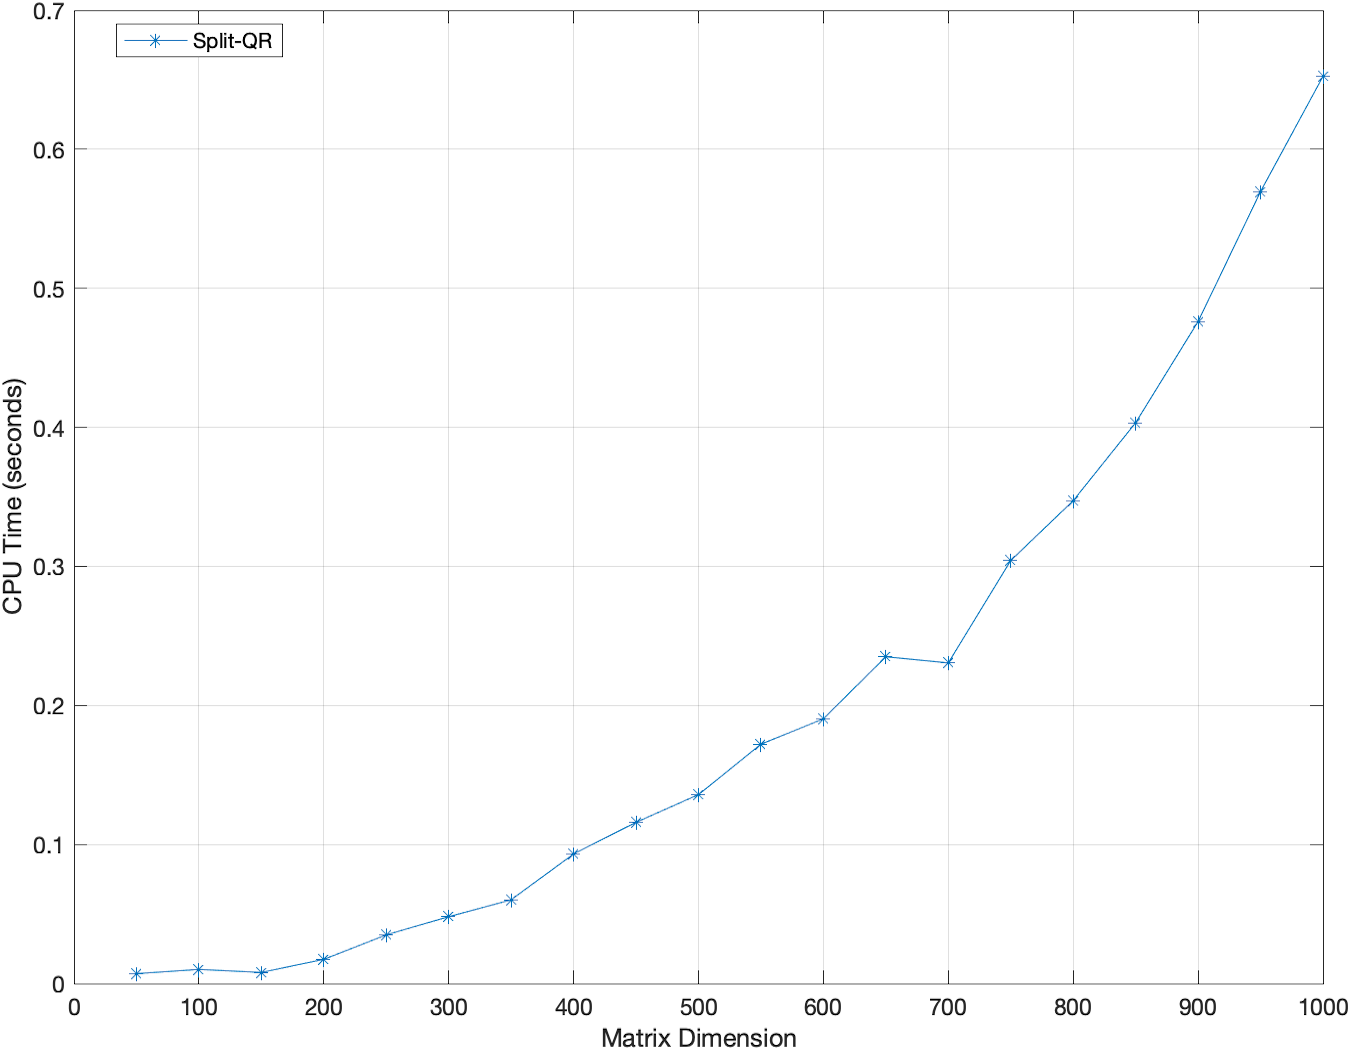
\includegraphics[width=\textwidth]{images/Figure_2.png} % 替换为实际图片路径
            % \caption*{CPU Time (seconds)}
        \end{minipage}
        \hfill
        \begin{minipage}[b]{0.45\textwidth}
            \centering
            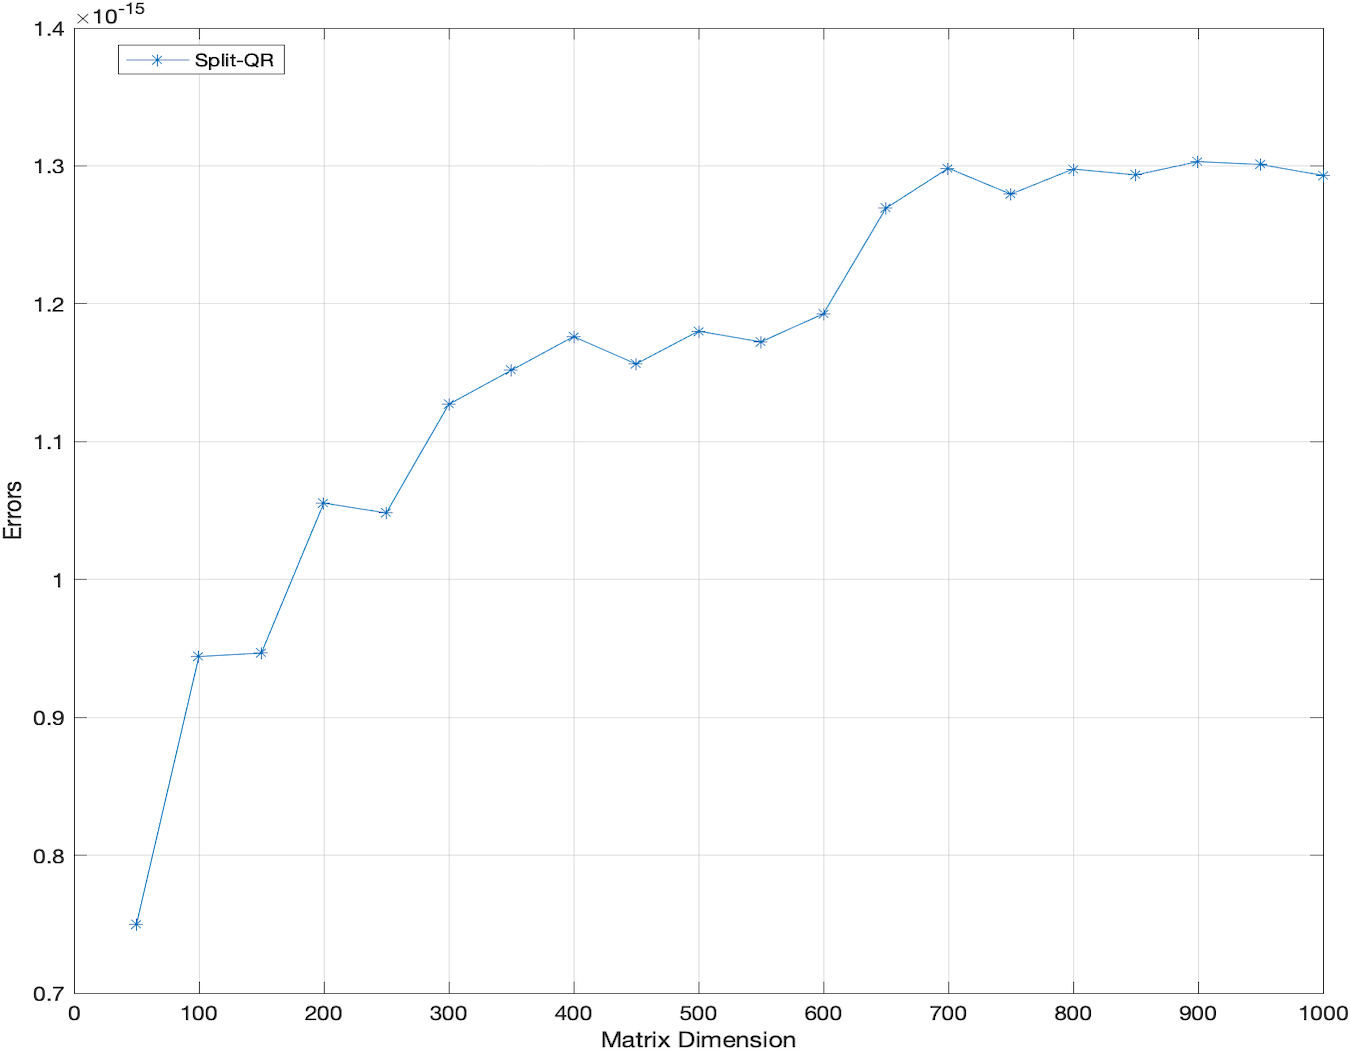
\includegraphics[width=\textwidth]{images/Figure_3.png} % 替换为实际图片路径
            % \caption*{Relative Error ($\log_{10}\epsilon$)}
        \end{minipage}
        \caption{Performance of \ref{alg:QR} on Random Matrices}
    \end{figure}
    \textbf{Conclusion:} The algorithm shows high efficiency and accuracy (errors around $10^{-15}$).
\end{frame}

% 实验2:矩阵方程求解
\begin{frame}
    \frametitle{Experiment 2: Solving Split Quaternion Matrix Equations}
    \textbf{Problem:} Solve \( AX = B \) where \( A,B \in \mathbb{H}_s^{3 \times 3} \) (explicit matrices given).
    
    \vspace{0.3cm}
    \textbf{Steps:}
    \begin{enumerate}
        \item Use \ref{alg:QR} to decompose \( A = QR \) (unitary \( Q \), upper triangular \( R \)).
        \item Transform the equation: \( QRX = B \implies RX = Q^H B \) (since \( Q^H Q = I \)).
        \item Solve \( RX = \widehat{B} \) (where \( \widehat{B} = Q^H B \)) via back substitution (due to \( R \) being upper triangular).
    \end{enumerate}
\end{frame}

% 实验2结果
\begin{frame}
    \frametitle{Experiment 2: Results}
    \begin{itemize}
        \item \textbf{QR Decomposition of \( A \):} Obtained \( Q \) (unitary) and \( R \) (upper triangular) explicitly.
        \item \textbf{Transformed RHS:} Computed \( \widehat{B} = Q^H B \).
        \item \textbf{Solution \( X \):} Solved via back substitution, with elements given explicitly.
        \item \textbf{Accuracy:} Relative error \( \frac{\|AX - B\|_F}{\|B\|_F} = 1.2412 \times 10^{-15} \) (high precision).
    \end{itemize}
    
    \vspace{0.3cm}
    \textbf{Conclusion:} QR decomposition provides an effective method for solving split quaternion matrix equations.
\end{frame}

% 结论概述
\begin{frame}
    \frametitle{Conclusion}
    \begin{block}{Key Contributions}
        1. Established a relationship between upper triangular matrices \( R \) and block matrices \( R_4 \) via permutations: \( R_4 = P_{2m} R P_{2n}^T \).
        
        2. Proposed an optimized permutation algorithm (\ref{alg:Permutation Optimization}) to efficiently transform \( R \) to \( R_4 \).
        
        3. Developed a special decomposition \( A^\sigma = \widetilde{Q} R_4 \) and derived \ref{alg:QR} for split quaternion QR decomposition.
        
        4. Verified the algorithm's efficiency and accuracy through numerical experiments and applications to matrix equations.
    \end{block}
\end{frame}

% 未来工作
\begin{frame}
    \frametitle{Future Work}
    The proposed method can be extended to other matrix decompositions for split quaternions:
    \begin{itemize}
        \item Schur decomposition.
        \item Eigenvalue decomposition.
        \item Singular value decomposition (SVD).
        \item Applications in more complex problems (e.g., least squares, control theory).
    \end{itemize}
\end{frame}

% 参考文献页(需要时添加)
\begin{frame}[allowframebreaks]{References}
  \printbibliography
\end{frame}

\end{document}


